
\subsubsection{Задача прогнозирования}
Подобно задаче $topN$, для решения задачи $pred$ \cite{cfrs, cf-expert,
rs-handbook, toward,coscial-rec-survey, user-item-cf,rs-cf}
строится кластер соседей, центром которого является активный пользователь
$u_a$, однако в кластер входят не только те пользователи, между которыми
и активным выполняется отношение близости, но и такие, которые оценили
прогнозируемый объект $i_{\bot}$:
$\nup = \{u: u_a \ru u \wedge \rho(u,i_{\bot}) \in P_0\}$. Такое дополнительное
условие накладывается для того, чтобы по известным $\rho(u, i_{\bot}), u \in \nup$
определить неизвестную $\rho(u,i_{\bot})$.
Следуя утверждению СОМ (\ref{assertSRS1}), $\forall$ $u \in \nup$ выполняется $|\rho(u_a,i_{\bot}) -
\rho(u,i_{\bot})| \le
\varepsilon_p$.
Для того, чтобы рассчитать прогнозную оценку,
вычисляется значение некоторой прогнозной функции $f_p$
от оценок, поставленных прогнозируемому объекту соседями:
\begin{equation}
	\rh(u_a,i_{\bot}) = f_p(\{ \rho(u,i_{\bot}): u \in \nup \})
\end{equation}

На рисунке (\ref{dia:nup}) изображена блок-схема алгоритма
построения кластера соседей $\nup$, которой соответствует псевдокод
(\ref{alg:nup}).
\begin{figure}[htb]
	\caption{Блок-схема алгоритма построения кластера $\nup$}
\begin{center}
	\label{dia:nup}
 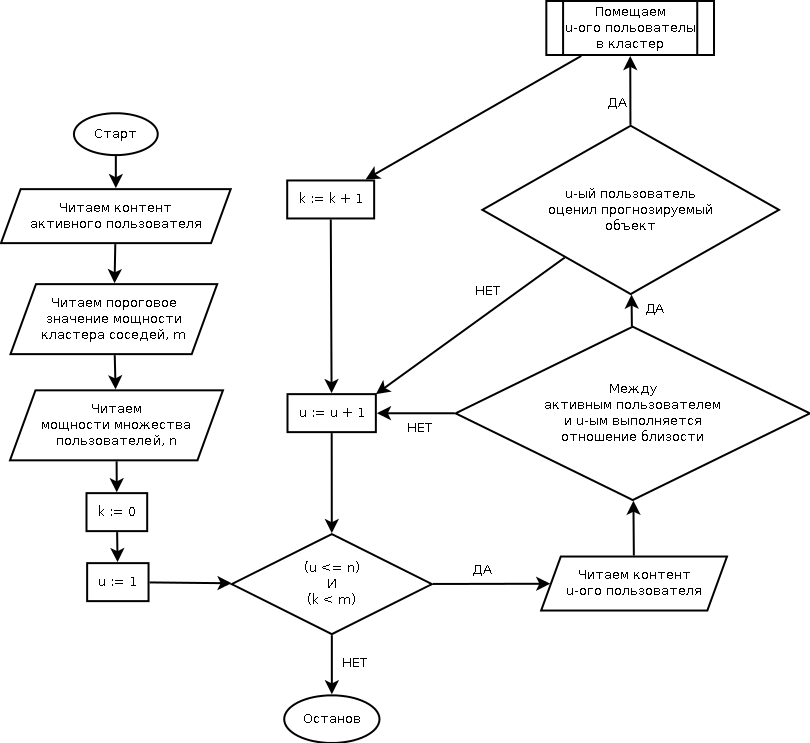
\includegraphics[width=7in,height=8in]{pics/algs/nup.png}
\end{center}
\end{figure}

\begin{figure}[htb]
	%\begin{algorithm}
		\caption{Построение множества соседей для активного
		пользователя при решении задачи прогнозирования в СОМ}
		\label{alg:nup}
		\begin{algorithmic}[1]
			\State $\nup \gets \varnothing$
			\State $k \gets 0$
			\For {$u \gets 1 \to |U|$}
			\If{($u_a \ru u$) $\wedge$ $(\exists$ $\rho(u, i_{\bot}))$}
			\State $\nup \gets \nup \bigcup \{ u \}$
			\State $k \gets k + 1$
			\EndIf
			\If{$k > M$}\Comment{Ограничение на размер множества соседей}
			\State Стоп
			\EndIf
			\EndFor
		\end{algorithmic}
	%\end{algorithm}
\end{figure}

Стандартный алгоритм решения задачи $pred$ в СОМ производится
в две итерации, которым соответствует псевдокод, представленный на изображении <<Стандартный алгоритм решения задачи прогнозирования в СОМ>>
 (\ref{alg:p-srs}):
\begin{enumerate}
	\item формирование кластера соседей $\nup$ (\ref{alg:nup});
	\item вычисление прогнозной функции по множеству оценок $\{\rho(u, i_{\bot}): u
		\in \nup\}$.
\end{enumerate}

\begin{figure}[htb]
	\caption{Стандартный алгоритм решения задачи прогнозирования в СОМ}
	\label{alg:p-srs}
		\begin{algorithmic}[1]
			\State $\nup$ \Comment{Формируем кластер соседей}
			\State $\rh(u_a, i_{\bot}) \gets f(\{\rho(u, i_{\bot}): u
			\in \nup\})$ \Comment{Вычисляем прогнозную функцию}
		\end{algorithmic}
\end{figure}
